\begin{center}
{\huge\textbf{\ttitle}}\\
\end{center}
\section{Introduction and background}
Today's world runs on internet. The demand for internet is increasing every second but infrastructure supporting internet is not scaling as fast. \\
A router is backbone of a network. It helps in transferring data. It is connected to some incoming links and some outgoing links. When combined bandwidth of incoming links exceed combined bandwidth of outgoing link, excess packets are stored in router's buffer but the router has finite buffer. When the buffer gets full router starts to drop packets, this scenario is called Congestion. Transmission Control Protocol (TCP) uses this implicit signal of dropping packets as sign of congestion. We can tune this packet dropping behaviour to notify clients of congestion early. We can do this using Active Queue Management (AQM) policies.\\ 
The router can drop packets when its buffer gets full but it creates a situation of bufferbloat i.e its buffer is never empty. To ensure that this situation doesn't occur Random Early Detection (RED) was developed. In RED, router starts to drop packets with some probability, the probability depends on the moving average of queue size. \\
Some of Active Queue Management (AQM) algorithms used in today's routers :
\begin{enumerate}
    \item Threshold Based Queuing: If queue size is beyond a threshold, the router starts to drop packets. % more details
    \item Random Early Detection: Router starts to drop packets with probability dependent on queue size i.e when queue is empty the probability is 0 and when queue is full the probability is 1 and in between it calculates the probability and drops packets.  % fill the examples
\end{enumerate}
Our goal in this project is to implement a Threshold based Active Queue Management (AQM) policy in a Network Simulator (ns-3).

\clearpage

%%%%%%%%%%%%%%%%%%%%%%%%%%%%%%%%%%%%%%%%%%%%%%%%%%%%%%%%%%%%%%%%%%
\section{Literature survey}
Transmission Control Protocol (TCP) is a reliable, in-order, byte-stream transport layer protocol \cite{rfc9293}. TCP reliability constitutes of error correction mechanism, detecting packet loss and correction via re-transmission \cite{rfc9293}. \\
TCP uses various congestion control mechanisms \cite{rfc5681} :
\begin{itemize}
    \item Slow Start: At start of a connection, transmission rate (Congestion window (cwnd) size) is increased exponentially until a threshold called slow start threshold (ssthresh) is reached or congestion is detected.
    \item Congestion Avoidance: After threshold is reached, TCP increases congestion window linearly
until bandwidth limit is reached.
    \item Fast Re-transmit and Fast Recovery: When packet loss is detected TCP re-transmits the package
and enter fast recovery to recover from the loss.
\end{itemize}
Some notable improvements include:
\begin{itemize}
    \item Reno \cite{rfc5681}: Improving fast Re-transmit and fast recovery aspect of TCP.
    \item NewReno \cite{rfc6582}: Improvement over Reno, improves re-transmission during fast-recovery phase of Reno. 
    \item Cubic \cite{rfc9438}: Uses cubic function instead of linear function for congestion window increase. It is designed for high speed and long distance network.
\end{itemize}
Routers has some finite buffer in which it stores the packets that it can't send immediately. Generally routers drop incoming packets when its buffer is full. But using, Active Queue Management (AQM) techniques it tries to manage buffer, dropping packets before buffer gets full or using a some criteria for dropping packets\cite{bachl22}. Random Early Detection (RED) is one such AQM where, when the average queue size exceeds a preset threshold the router drops incoming packet with a certain probability, where exact probability is a function of the average queue size \cite{floyd93}. RED is highly dependent on initial parameter setting and is not well performant with bursty traffic. Various changes have been suggested to RED such as Exponential RED \cite{shao05}, PIE \cite{pan13} etc. While in Threshold based queueing policy router drops incoming packet when queue size exceeds a certain threshold. Some disadvantages of threshold based queueing policy are burst losses i.e all packets are dropped suddenly, flow synchronization i.e all flows are either backing off simultaneously or sending packets simultaneously. To detect flow synchronization at routers we have use method described here \cite{hass08}. To get a number that defines synchrony between two flows. We have also used a method of analysing queue size at router to detect synchronization. \\ 

\clearpage
\section{Problem definition and Objective}
TCP sends multiple packets at the same time. The set of packets is called sending window or cwnd. TCP changes the size of cwnd during different states it is in, like slow start, congestion avoidance. In congestion avoidance phase of TCP, it follows additive increase and multiplicative decrease (AIMD) to change cwnd size. \\
Additive increase: \( w_{t+1} = w_{t} + \alpha w_{t}^{k-1} \)\\
Multiplicative decrease: \( w_{t+1} = (1-\beta)w_{t}  \)\\
where \( \alpha > 0, \beta < 1 \) and \( k \) determines the nature of additive increase.\\
The value of \( q_{th} \) can be calculated as \cite{manjunath2019compound}: \\ 
\[
    \beta w^* \left(\frac{w^*}{C \tau}\right)^{q_{th}}{q_{th}} = \pi/2
\]
where $ q_{th} $ is queueing threshold, \textit{C} is link bandwidth, $ \tau $ is one divided by average round trip time, $ \beta $ is AIMD parameter (generally 0.5) and $ w^* $ is average window length.\\
Now, how to calculate the parameter \( q_{th} \) effectively.  \\
To calculate of $ q_{th} $ we require values of $ \beta $ and $ w^* $. \\
So, the objective of our project is to: 
\begin{enumerate}
    \item Simulate sample topologies in ns-3 and generate data
    \item Calculate \( \beta \) value and $ w^* $ from generated data, then calculating \( q_{th} \) 
    \item Implement this whole process of calculating $ q_{th} $ then setting it as threshold, in ns-3 
\end{enumerate}

\clearpage

\section{Methodology}
The methodology we took to achieve the desired objective:
\begin{figure}[h]
    \centering
    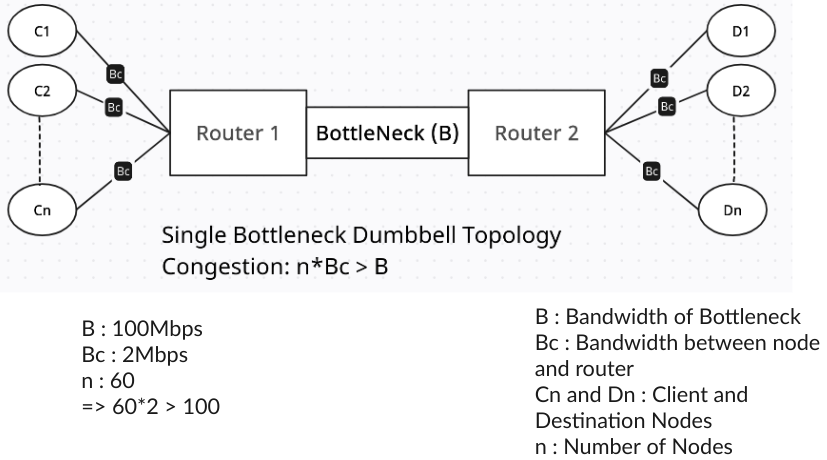
\includegraphics[width=0.55\textwidth]{./images/topology.png}
    \caption{\label{fig:myfig2} Topology used for Simulation}
\end{figure}
\begin{enumerate}
    \item Literature Review: We have done extensive literature review on our topic. By doing this we found at what level current state of the art is. We also learnt about different approaches explored to counter network congestion.
    \item ns-3: ns-3 is a network simulator program. It is open-source so anybody can contribute in it. It is used to simulate different network scenarios. It uses C++ Programming language at is base. The topology can be build using C++ code. It is a network simulator so all the pieces required for simulating a network scenario exist in it. We learnt how to use ns-3 to simulate example topology.
    \item Topology Generation: The parameters given in the image \ref{fig:myfig2} satisfies the congestion scenario i.e combined bandwidth of incoming links should be greater than combined bandwidth of outgoing links. Using C++ code we simulated this topology in ns-3.
    \item Learning About Congestion Control: We learnt about different TCP flavors like TCP Tahoe, Reno, NewReno, Cubic etc. How they handle congestion, their disadvantages and disadvantages, use cases etc. We also learnt about how routers handle congestion different packet dropping policies and how they impact current internet.
    \item Generating Data: By simulating given network topology we generated that can be used for further analysis.
    \item Understanding data: At this phase, we basically analyzed the generated data what different inferences we can generate from it.
    \item Finding Optimal Parameters: We propose using data driven approach to calculate \( \beta, \alpha \) and \( k \) values, and from that we can calculate value of \( q_{th} \). 
    \item Updating the metric: In this phase we will be implementing our approach in ns-3. Comparing our results with with general congestion scenario and check if our approach fairs better or worse.
    \item Benchmarking: We analyze the performance of our model.
\end{enumerate}

\clearpage
\section{Theoretical/Numerical/Experimental findings}
The result is generated using simulation for the given topology (\ref{fig:myfig2}). Trace file at router 1 was collected as well as change of cwnd size with time for each client node was also collected. 

Some of the result is discussed below:\\
\begin{figure}[h]
    \centering
    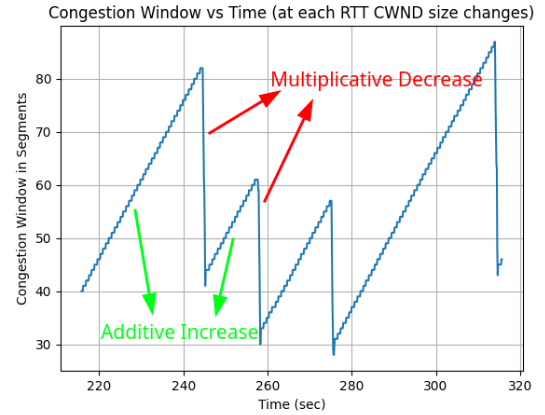
\includegraphics[width=0.55\textwidth]{./images/aimd.png}
    \caption{\label{fig:myfig3} Congestion window (\textit{w}) vs time for one node}
\end{figure}
\begin{figure}[h]
    \centering
    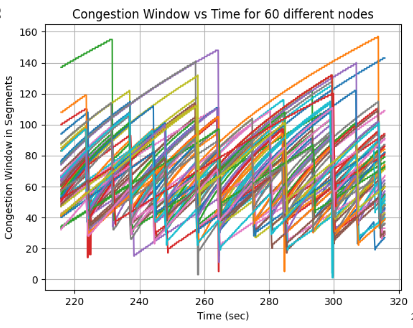
\includegraphics[width=0.55\textwidth]{./images/allNodesCwnd.png}
    \caption{\label{fig:myfig4} Congestion Window (\textit{w}) vs time for all nodes}
\end{figure}
\begin{figure}[h]
    \centering
    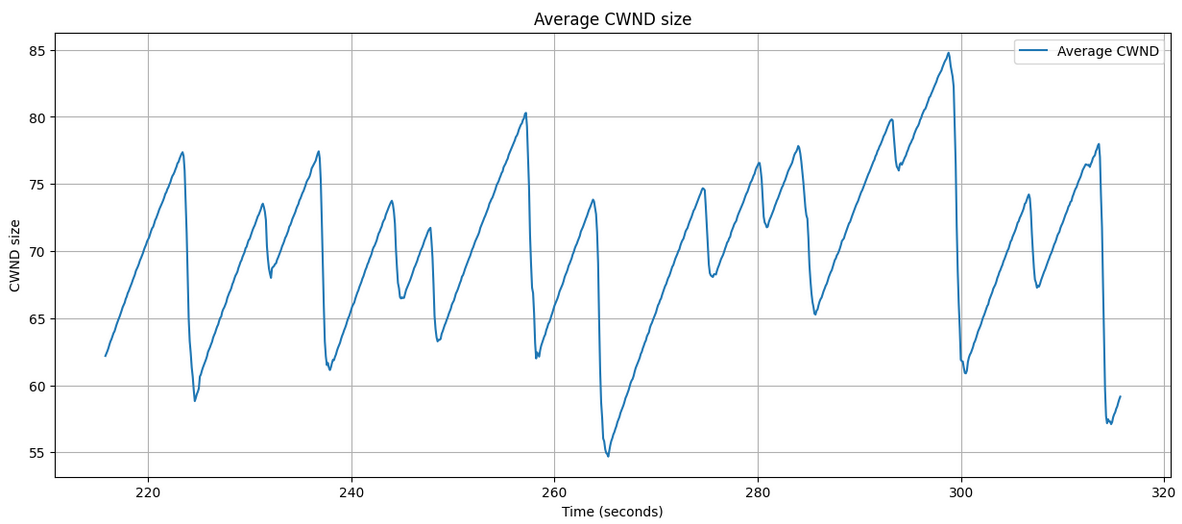
\includegraphics[width=0.55\textwidth]{./images/avgCwnd.png}
    \caption{\label{fig:myfig5} Average Congestion Window (\textit{w*}) vs time }
\end{figure}
1. This graph (\ref{fig:myfig3}) shows how cwnd size varies with time for a single node. You can see in this graph how additive increase and multiplicative decrease (AIMD) works in congestion avoidance phase of TCP. Size of cwnd either increases linearly or decreases multiplicatively with each RTT in congestion avoidance phase.\\ % graph 
2. This graph (\ref{fig:myfig4}) shows cwnd size vs time for all 60 nodes. This graph shows how global synchronization leads to bandwidth under utilization. Global synchronization means either all nodes send traffic simultaneously or back off simultaneously. \\ % graph
3. This graph (\ref{fig:myfig5}) show average cwnd ($ w^* $) vs time. $ w^* $ is average of $ w $ for all nodes with time. \\ %graph
4. This graph (\ref{fig:myfig6}) shows how we have found synchronization between two flows. Due to results being inconclusive for when AQM is on and when AQM is off we didn't go further with it. \\ 

\begin{figure}[h]
  \centering
  \includegraphics[width=0.8\textwidth]{assets/2025-05-06-10-53-43.png}
  \caption{Loss synchronization between pair of flows}
  \label{fig:myfig6}
\end{figure}

\begin{figure}[h]
  \centering
  \includegraphics[width=0.8\textwidth]{assets/2025-05-06-11-06-53.png}
  \caption{Queue Size vs Time}
  \label{fig:myfig7}
\end{figure}

\begin{figure}[h]
  \centering
  \includegraphics[width=0.8\textwidth]{assets/2025-05-06-11-07-37.png}
  \caption{Autocorrelation of Queue Size}
  \label{fig:myfig8}
\end{figure}
5 . This graph (\ref{fig:myfig7}) shows our approach to find trigger condition. We see queue size vs time for queue size 2084 and 30. In queue size 2084 case we see there is some pattern. When we calculate its autocorrelation (\ref{fig:myfig8}) we see that for some overlap autocorrelation is high. Then we find number of zero crossings from it. When number of zero crossings is less than a threshold we trigger AQM. \\ 



6. Some results after simulations are depicted in figure \ref{fig:myfig9}, \ref{fig:myfig10}, \ref{fig:myfig11}, \ref{fig:myfig12}. For flow completion time calculation, 100MB data is transferred otherwise data is unbounded. You can see in the graphs while average throughput is less for AQM case, we can see that it can take values between two whiskers (standard deviation) which can be greater than No AQM case sometimes. Same for other graphs. \\ 

\begin{figure}[h]
  \centering
  \includegraphics[width=0.8\textwidth]{assets/2025-05-12-10-16-44.png}
  \caption{Average Throughput vs RTT}
  \label{fig:myfig9}
\end{figure}

\begin{figure}[h]
  \centering
  \includegraphics[width=0.8\textwidth]{assets/2025-05-12-10-17-26.png}
  \caption{Queueing Delay vs RTT}
  \label{fig:myfig10}
\end{figure}
 
\begin{figure}[h]
  \centering
  \includegraphics[width=0.8\textwidth]{assets/2025-05-12-10-18-41.png}
  \caption{Flow Completion Time vs RTT}
  \label{fig:myfig11}
\end{figure}

\begin{figure}[h]
  \centering
  \includegraphics[width=0.8\textwidth]{assets/2025-05-12-10-18-09.png}
  \caption{Packet loss vs RTT}
  \label{fig:myfig12}
\end{figure}


\clearpage
\section{Summary and Future plan of work}
In our project we aim to propose a solution to widely encountered situation in today's internet connected world, Network Congestion. Congestion wastes important resources such as time, computing power etc. If not handled properly it can lead to collapse of whole internet infrastructure. It occurs in routers, when incoming traffic is greater then bandwidth of outgoing link. Routers have finite buffer that they use to continuously send data thus utilizing full bandwidth. Most of recent work is focused on making end points more intelligent and handling congestion mainly through them. Active Queue Management (AQM) serves as a way for router to control congestion as well as notify end points that a congestion has occurred or it is likely to occur if they don't lower their sending rates. Random Early Detection (RED) randomly starts to drop packets as queue get full. While Threshold based queuing policy starts to drop packets when queue size crosses a certain threshold. In our project we aim to modify threshold based queuing policy such that it ensures stability as well as greater throughput thus more utilization of bandwidth.\\
In the results we see that while our AQM did not performed better than network without AQM, its performance was not much worse. So, while utilising minimal resource performance can sometimes be better than No AQM case. \\ 
Future work includes refining our approach as well as finding new ways to accomplish the project's objective. \\

\clearpage

%\section*{Publications  (if any)}
%\addcontentsline{toc}{section}{Publications  (if any)}
%\myemptypage

%\section*{Appendix (if any)}
%\addcontentsline{toc}{section}{Appendix (if any)}
